\documentclass[11pt, titlepage]{article}
\usepackage[pdftex]{graphicx}
\usepackage{mathtools}
\usepackage{amsthm}
\usepackage{amssymb}
\usepackage{microtype}
\usepackage{parskip}
\makeatletter
\renewcommand\@seccntformat[1]{}
\makeatother

\author{Graeme Douglas (76316090)}

\begin{document}

\section{Use Case Diagram}
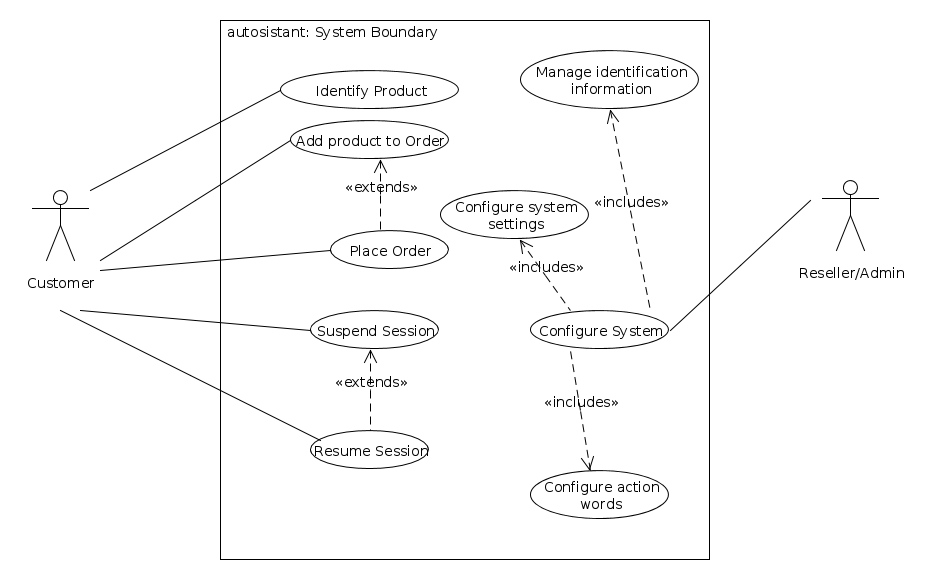
\includegraphics[scale=0.42]{project_usecasediagram.png}
\subsection{Summary of Use Case Diagram}
The following is a summary of the use cases in the above diagram for the
``Customer'' actor.
\begin{itemize}
\item \textbf{Identify Product}.  The user may search for and identify
products so that they may check product stock, find its price, or add products
to the user's order.
\item \textbf{Add product(s) to Order}.  When a customer has several items to
choose from, the system should give the user a choice.  The user should be able
to choose zero, one, or many of these products.
\item \textbf{Place Order}.  A customer should have the option to place an
order for the products they have chosen.  This should be handled with in the
chat system.
\item \textbf{Suspend session}.  A costumer should be able to suspend a session.
This way, a customer can leave part way through setting up an order, should they
need to, and later resume the session.  The system will return an identification
token that the user can use to return to the previous session.
\item \textbf{Resume session}.  Should a customer be disconnected at some point,
either by choice or because of some technical glitch, they should able to
resume the previous session, so long as the reconnection occurs within a given
period of time, defined by the system administrator / reseller.
\end{itemize}
The following is a summary for the uses cases for the ``Reseller'' actor.
\begin{itemize}
\item \textbf{Configure system}.  The reseller must be able to tune various
aspects of the system.  This includes the following use cases:
\begin{itemize}
\item \textbf{Manage identification information}.  This allows the reseller
to add the ways a customer can identify a specific product.  For example,
if a reseller sold a dish washers, some ways of identifying a product is to
search via brand or warranty period.  The reseller or system administrator
must be able to both configure these categories and what values these categories
take on for various products.
\item \textbf{Manage company information}.  This includes information like the
company's name.
\item \textbf{Configure action words}.  An administrator must be able to
configure what words trigger certain system actions.  One reseller might
desire for the word ``buy'' to trigger a product identification action,
while another reseller might want the same word to be a confirmation
signifier.
\end{itemize}
\end{itemize}

\end{document}

